\section{Introduction}

3D Gaussian Splatting (3DGS) provides a high-quality and efficient
representation for reconstructing and rendering three-dimensional
environments. Its ability to represent both scene geometry and
appearance makes it attractive for long-term applications such as
robotic mapping and augmented reality. In these applications, however,
the environment may change over time: objects can be added, removed,
or moved, and local appearance can vary between mapping sessions.
When a mapping system updates its representation using new
observations, overwriting the previous map may erase the last recorded
state of the environment. Preserving historical map versions would
support applications such as querying past scenes, restoring earlier
maps, comparing recorded states, and evaluating mapping algorithms
against previously constructed maps.

Existing methods address several aspects of evolving scenes, but
they provide different guarantees for historical access. Online
mappers such as GaME~\cite{yugay2026game} adapt the current map by
adding new geometry, removing outdated Gaussians, and suppressing
stale observations. Continual methods provide additional support for
scene history: CL-Splats~\cite{ackermann2025clsplats} recovers past
states by recording local changes, while
GaussianUpdate~\cite{zeng2025gaussianupdate} and
LTGS~\cite{kim2026ltgs} represent past scenes using Gaussian visibility
and shared object templates, respectively. These approaches support
map updates or historical rendering through specific update rules or
shared scene representations. Dynamic Gaussian
representations~\cite{luiten2024dynamic,wu2024gaussians} also enable
rendering at different timestamps through trajectories or
time-conditioned deformations. However, the ability to query a
timestamp does not by itself guarantee that a previously committed
map state remains unchanged after subsequent optimization.

A straightforward way to preserve immutable states is to store each
map version as an independent snapshot. This approach permits direct
access and exact recovery, but its storage cost grows with the
cumulative size of all versions. Delta-based storage can reduce
redundancy, yet cross-version parameter correspondence becomes
difficult when Gaussian topology changes. Moreover, recovering a
version from a chain of deltas may require applying intermediate
updates. Thus, it remains challenging to preserve immutable Gaussian
map versions, share storage across updates, and directly replay any
committed version.

Achieving these properties requires addressing two related challenges.
First, Gaussians do not have stable identities by default.
Densification creates Gaussians through cloning and splitting, while
pruning and scene updates remove existing ones. These operations
change the number and ordering of Gaussians, so a tensor row cannot
reliably identify the same Gaussian across versions. Second, parameter
changes do not necessarily correspond to changes in the scene.
Continued optimization may adjust the positions, shapes, and
appearance of Gaussians even in regions where the environment has
remained unchanged. Preserving every such parameter update limits
cross-version sharing, whereas reusing earlier parameters may affect
the quality of the newly committed map. A versioning system must
therefore track Gaussians across topology-changing updates and decide
which parameters can be reused while accounting for their effect on
map quality.

% \begin{center}
% 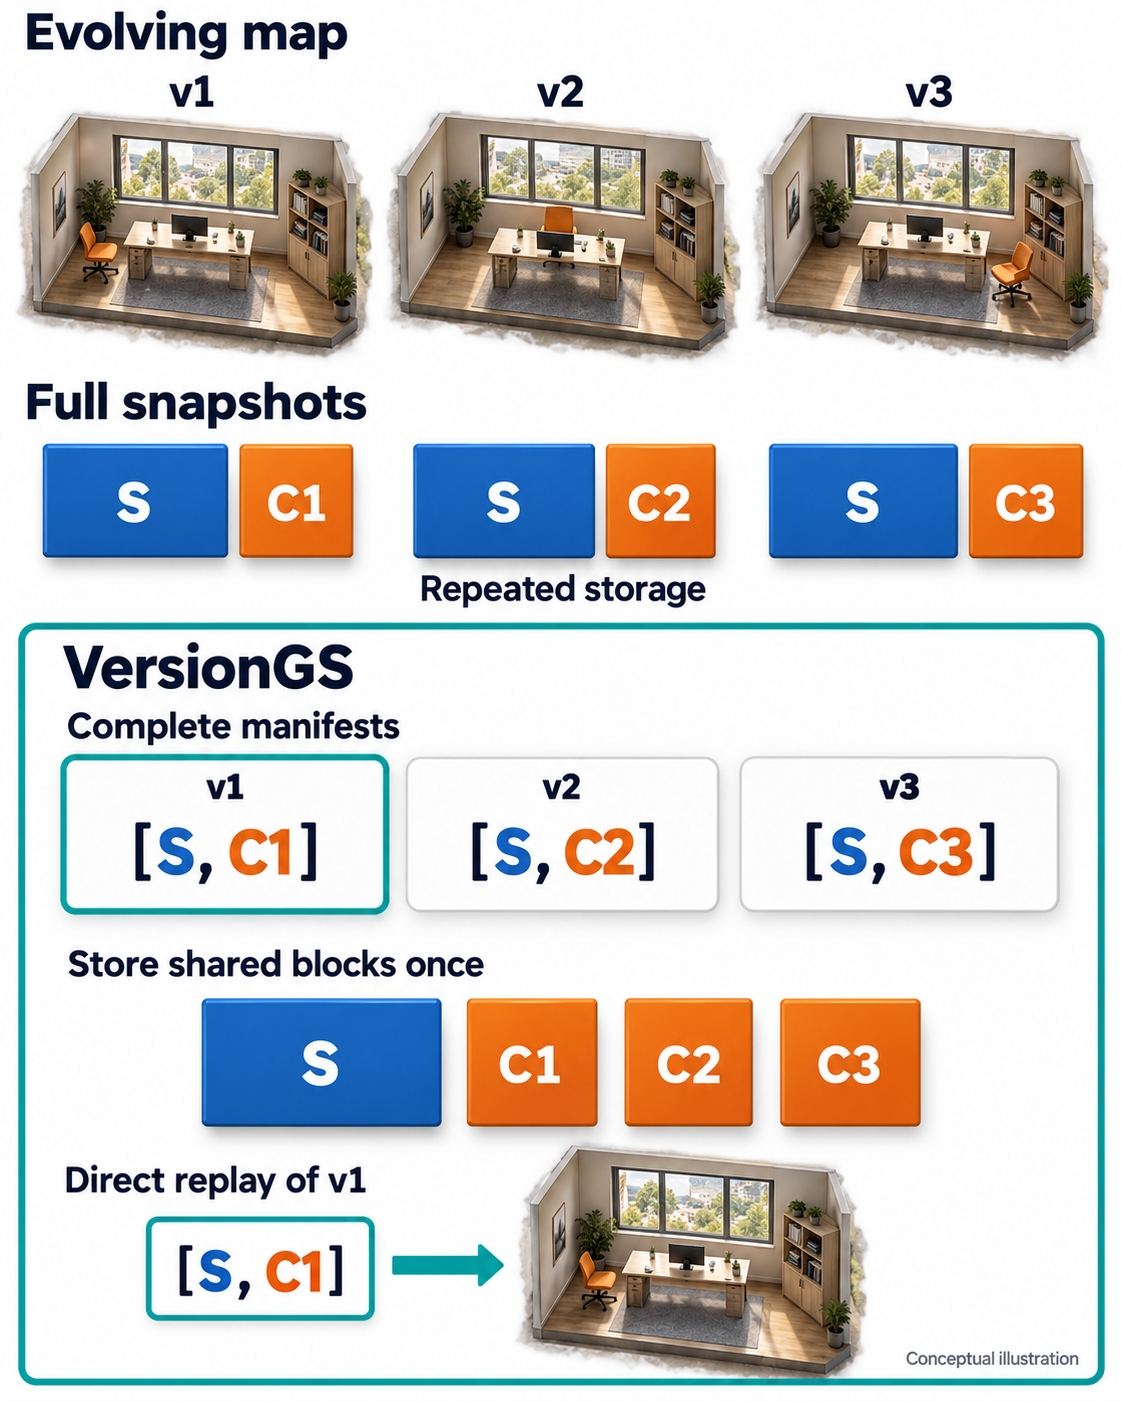
\includegraphics[width=\columnwidth]{section/01_TeaserFigure.png}
% \end{center}




To address these challenges, we present \textbf{VersionGS}, a
framework for archiving and replaying evolving 3D Gaussian maps.
Its central design is to make every committed version logically
complete while sharing identical content across versions in physical
storage. VersionGS separates the live map being optimized from its
committed versions, so subsequent updates do not alter earlier
commits. It assigns persistent identities to Gaussians, allowing
them to be tracked across updates even when their tensor rows change.
When constructing a new version, VersionGS uses scene-change evidence
and visibility to select parameters from the current map or reuse
parameters from the previous commit. New Gaussians and regions
identified as changed use current parameters; for other regions,
the framework reuses earlier parameters where possible and checks
rendering quality to limit the impact of reuse.

\begin{figure}[H]
\centering
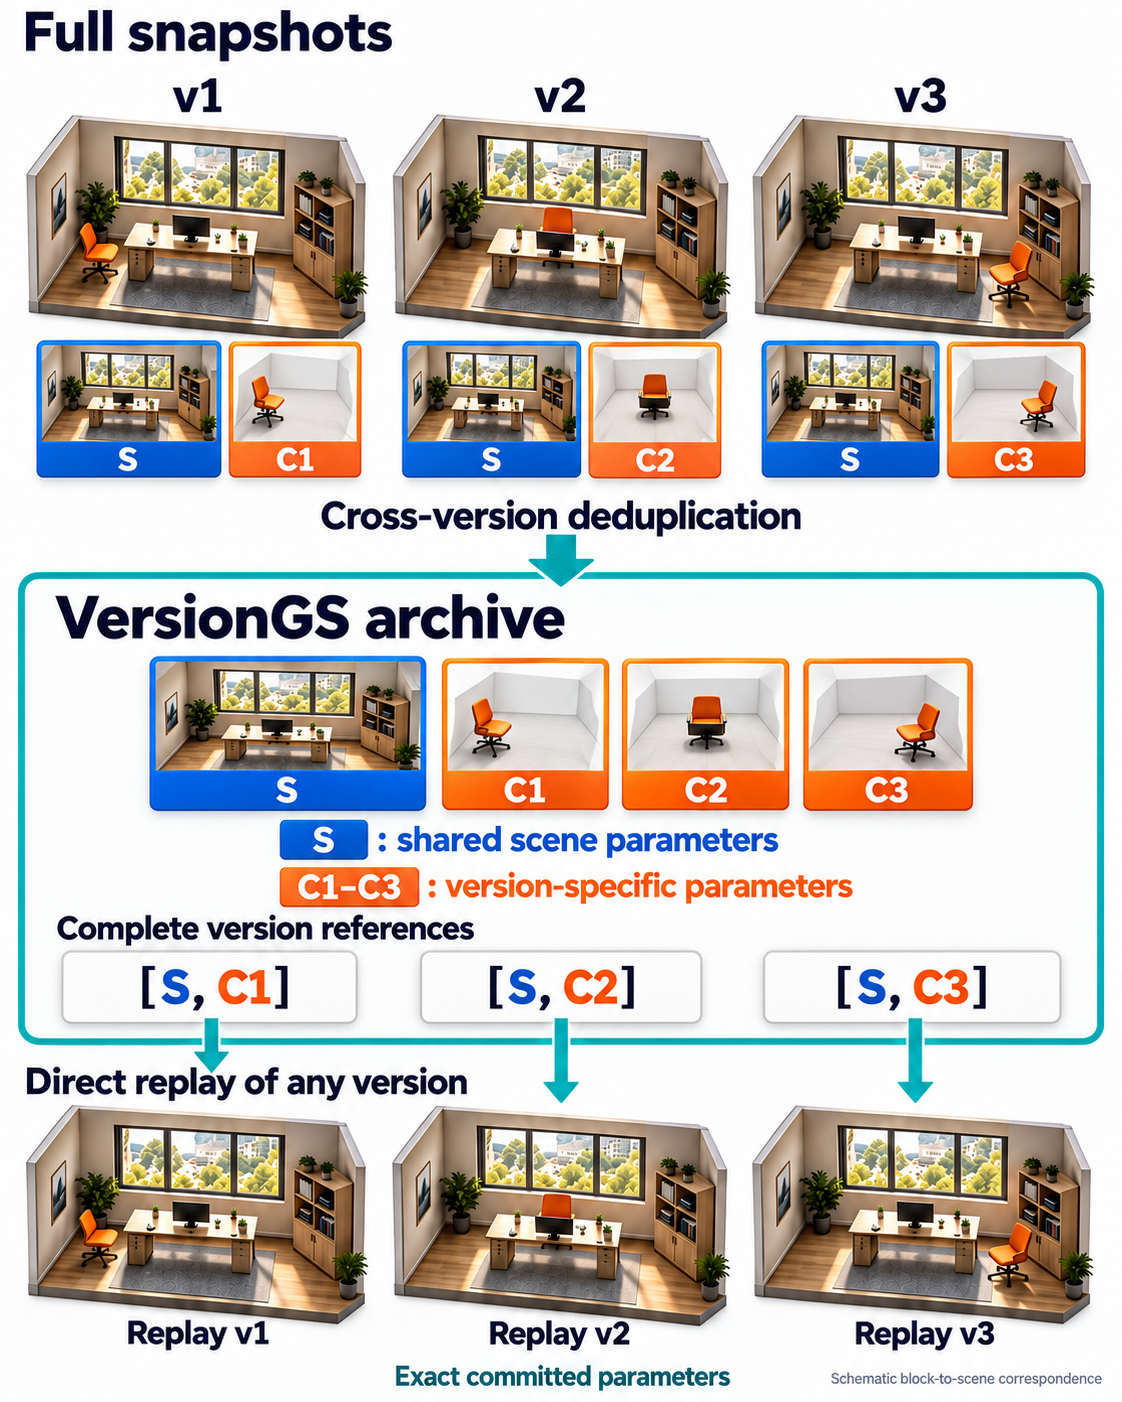
\includegraphics[width=\columnwidth]{figures/01_TeaserFigure_v3.png}
\caption{Example Image}
\label{fig:example}
\end{figure}

The resulting committed version may therefore differ from the live
map. Once committed, however, its selected parameters are stored
losslessly. Each version is represented by a complete manifest of
references to Gaussian parameter blocks, and identical blocks are
stored only once through content addressing. This design enables
exact recovery and direct rendering of any committed version without
the original observations or replaying intermediate updates.

We evaluate VersionGS on [datasets] across [number] successive map
versions. Our experiments measure the rendering quality of current
and historical versions, total archive storage, and the time required
to save and load a version. We compare against full snapshots,
compressed snapshots, and delta-based storage to evaluate the
benefits and costs of cross-version sharing. VersionGS reduces
archive storage by [X] compared with [baseline], while keeping
current-version rendering quality within [Y] dB of the underlying
mapper. We also verify that committed parameters are recovered
exactly and that historical versions remain unchanged after further
map updates.

Our contributions are threefold:
\begin{enumerate}
    \item We formulate the problem of archiving evolving 3D Gaussian
    maps as immutable, directly accessible versions despite
    topology-changing updates.

    \item We introduce persistent Gaussian identities and a
    change-aware version construction method that uses change
    evidence, visibility, and rendering-quality checks to guide
    parameter reuse across versions.

    \item We develop a lossless multi-version archive based on
    complete version manifests and content-addressed Gaussian
    parameter blocks, enabling exact replay of committed versions
    without the original observations or intermediate updates.
\end{enumerate}